\chapter{Austauschsymmetrie, Spin und die beiden Minuszeichen}

\section{Schalenbesetzung und die Frage nach der Spin--Statistik}

Die Betrachtung des Schalenmodells beginnt mit zwei Eigenschaften der Elektronen. Ein Elektron hat den Spin eins halb, mit den beiden dimensionslosen Spinprojektionen
\begin{equation}
m_s=+\frac12,
\qquad
m_s=-\frac12,
\end{equation}
und Elektronen gehorchen dem Pauli-Ausschlussprinzip. Diese Tatsachen hängen zusammen, sind aber nicht dieselbe Aussage.

Der Ausdruck ``derselbe Zustand'' bedarf einer Präzisierung. Keine zwei Elektronen dürfen denselben vollständigen Einteilchenzustand besetzen. Zwei Elektronen können dennoch dasselbe räumliche Orbital teilen, wenn ihre Spinzustände verschieden sind. In der Näherung unabhängiger Elektronen für Helium besetzen beide Elektronen das niedrigste räumliche Orbital, eines mit Spin nach oben, das andere mit Spin nach unten. Genauer gesagt gehören die Alternativen ``das erste hat Spin nach oben und das zweite nach unten'' und ``das erste hat Spin nach unten und das zweite nach oben'' zu einem verschränkten Zweielektronen-Spinzustand.

Dies ist lediglich die alte Näherung des Schalenmodells. Sie vernachlässigt die Wechselwirkung zwischen den Elektronen und dient hier der einfachen Zählung. Bei Lithium besetzen die ersten beiden Elektronen das niedrigste räumliche Orbital mit entgegengesetztem Spin. Das dritte Elektron kann keinen dieser vollständigen Zustände einnehmen und muss ein höheres Orbital besetzen.

Als Nächstes folgt das vertraute Diagramm des Bahndrehimpulses. Die Bereiche mit
\begin{equation}
\ell=0,\qquad \ell=1,\qquad \ell=2
\end{equation}
heißen \(S\)-, \(P\)- und \(D\)-Zustände. Zu einem festen Wert von \(\ell\) gehören
\begin{equation}
2\ell+1
\end{equation}
Bahndrehimpulszustände, also
\begin{equation}
\ell=0\Rightarrow 1,
\qquad
\ell=1\Rightarrow 3,
\qquad
\ell=2\Rightarrow 5.
\end{equation}
Das Coulomb-Problem weist zusätzliche Entartungen auf: Radialzustände aus verschiedenen \(\ell\)-Sektoren können dieselbe Energie haben. Für die Betrachtung der Schalenbesetzung enthält die nächste Schale ein \(S\)-Orbital und drei \(P\)-Orbitale. Sie hat daher
\begin{equation}
1+3=4
\end{equation}
räumliche Zustände. Der Spin verdoppelt diese Zahl:
\begin{equation}
2(1+3)=8.
\end{equation}

Diese acht vollständigen Einteilchenzustände werden in der einfachen Abfolge von Lithium bis Neon aufgefüllt. Nach der abgeschlossenen Schale hat Natrium wieder ein äußeres Elektron; deshalb ähnelt es in diesem groben Bild Lithium. Um die Chemie geht es hier nicht. Entscheidend ist, dass halbzahliger Spin und Ausschluss gemeinsam auftreten.

Photonen bilden den Gegenfall. Sie haben ganzzahligen Spin und unterliegen keiner Ausschlussregel. Einer klassischen elektromagnetischen Welle entsprechen viele Photonen, die denselben Modus besetzen. Bosonen können sich in einem gemeinsamen Zustand ansammeln, während identische Fermionen einen vollständigen Zustand höchstens einmal besetzen können. Die Frage ist, ob diese beiden Zuordnungen auch andersherum möglich sein könnten: halbzahligen Spin ohne Ausschluss oder ganzzahligen Spin mit Ausschluss. In drei räumlichen Dimensionen lautet die Antwort gemäß der Spin--Statistik-Beziehung nein. Die vertraute Aussage bedarf in einer und zwei räumlichen Dimensionen einer Einschränkung; ein Beweis des feldtheoretischen Ergebnisses wird hier nicht versucht.

\begin{classroomqa}
\lecturetimestamp{00:11:48}
\audiencequestion{Gibt es eine Höchstzahl an Bosonen, die einen Zustand besetzen können?}
\lecturerresponse{Nein. Für Bosonen gibt es keine Besetzungsgrenze, und sie sammeln sich tendenziell im selben Zustand an.}
\end{classroomqa}

\section{Wellenfunktionen vieler Teilchen}

Dem Zusammenhang nähern wir uns über zwei Minuszeichen: eines stammt vom Austausch, das andere von der Rotation. Wir beginnen mit dem Austausch und lassen den Spin zunächst außer Betracht.

Sei \(x_i\) die Position des Teilchens \(i\). Der Index bezeichnet ein Teilchen und keine kartesische Komponente; die drei räumlichen Koordinaten werden in einem einzigen Symbol zusammengefasst: \(x_i\). Eine Ortsbasis für \(n\) Teilchen ist
\begin{equation}
\lvert x_1,x_2,\ldots,x_n\rangle.
\end{equation}
Für einen abstrakten Zustand \(\lvert\Psi\rangle\) lautet die Ortswellenfunktion
\begin{equation}
\psi(x_1,x_2,\ldots,x_n)
=
\langle x_1,x_2,\ldots,x_n\mid\Psi\rangle.
\end{equation}
Ihr Betragsquadrat,
\begin{equation}
\bigl\lvert\psi(x_1,x_2,\ldots,x_n)\bigr\rvert^2,
\end{equation}
ist die gemeinsame Wahrscheinlichkeitsdichte dafür, Teilchen \(1\) bei \(x_1\), Teilchen \(2\) bei \(x_2\) und so weiter zu finden.

Nehmen wir nun an, die Teilchen seien identisch. Stellen wir uns zunächst vor, ein Elektron sei blau und ein anderes rot angemalt. Dann ließe sich ``blau bei \(x_1\), rot bei \(x_2\)'' von ``blau bei \(x_2\), rot bei \(x_1\) unterscheiden.'' Tatsächliche Elektronen tragen keine solchen Farben oder individuellen Kennzeichnungen. Eine Vertauschung der Buchführungsindizes kann keine neue physikalische Anordnung erzeugen.

Eine globale Phase ändert weder Wahrscheinlichkeiten noch Erwartungswerte. Für einen Zustand mit bestimmtem Austauschverhalten kann die Ortswellenfunktion daher folgende Beziehung erfüllen:
\begin{equation}
\psi(x_2,x_1)=\eta\,\psi(x_1,x_2),
\qquad
\lvert\eta\rvert=1.
\end{equation}
Wendet man denselben Austausch zweimal an, erhält man die ursprünglichen Argumente zurück und es gilt
\begin{equation}
\eta^2=1,
\end{equation}
Die beiden möglichen Austauscheigenwerte sind somit
\begin{equation}
\eta=+1
\qquad\hbox{or}\qquad
\eta=-1.
\end{equation}

\editorialnote{Die Algebra des doppelten Austauschs legt die möglichen Eigenwerte erst fest, nachdem für einen Zustand ein bestimmtes Austauschverhalten vorausgesetzt wurde. Die weitergehende Einschränkung, dass die zulässigen Zustände einer festen Teilchensorte zu einem einzigen Austauschsektor gehören, ist eine physikalische Regel; sie folgt nicht allein aus \(\eta^2=1\). Dieselbe Einschränkung gilt für das folgende Ausschlussargument: Antisymmetrie impliziert Ausschluss, sobald der fermionische Sektor gewählt ist, aber die Algebra des Austauschs allein wählt diesen Sektor nicht aus.}

Bei Bosonen sind die zulässigen Wellenfunktionen symmetrisch,
\begin{equation}
\psi_B(x_1,x_2)=\psi_B(x_2,x_1),
\end{equation}
bei Fermionen dagegen antisymmetrisch,
\begin{equation}
\psi_F(x_1,x_2)=-\psi_F(x_2,x_1).
\end{equation}
Das Minuszeichen bleibt unsichtbar, wenn es den gesamten Zustand multipliziert, spielt aber eine Rolle, wenn Amplituden addiert werden. So hat die Austauschsymmetrie beobachtbare Folgen.

\section{Produkte, Summen und Ausschluss}

Betrachten wir zunächst zwei Teilchen, die demselben Einteilchenorbital \(\psi_0\) zugeordnet sind. Ihr Produkt lautet
\begin{equation}
\psi_0(x_1)\psi_0(x_2).
\end{equation}
Beim Austausch der Teilchenkoordinaten ergibt sich
\begin{equation}
\psi_0(x_2)\psi_0(x_1)
=
\psi_0(x_1)\psi_0(x_2).
\end{equation}
Wellenfunktionswerte sind Zahlen, keine Operatoren; die Faktoren kommutieren also. Das Produkt für denselben Zustand ist symmetrisch. Es ist eine zulässige bosonische Form, kann aber keine zwei identischen Fermionen beschreiben.

Ordnen wir die Teilchen nun verschiedenen Einteilchenorbitalen zu:
\begin{equation}
\psi_0(x_1)\psi_1(x_2).
\end{equation}
Beim Austausch erhält man
\begin{equation}
\psi_0(x_2)\psi_1(x_1).
\end{equation}
Für verschiedene Funktionen ist das vertauschte Produkt im Allgemeinen weder der ursprüngliche Ausdruck noch dessen Negatives. Das bloße Produkt besitzt daher keine der erforderlichen Austauschsymmetrien. Damit ist nicht ausgeschlossen, dass ein Teilchen \(\psi_0\) besetzt und ein anderes \(\psi_1\). Es bedeutet, dass der Zweiteilchenzustand die beiden Zuordnungen kombinieren muss.

Die symmetrische Kombination lautet
\begin{equation}
\psi_B^{(01)}(x_1,x_2)
\propto
\psi_0(x_1)\psi_1(x_2)
+
\psi_0(x_2)\psi_1(x_1),
\end{equation}
die antisymmetrische Kombination
\begin{equation}
\psi_F^{(01)}(x_1,x_2)
\propto
\psi_0(x_1)\psi_1(x_2)
-
\psi_0(x_2)\psi_1(x_1).
\end{equation}
Proportionalitätszeichen genügen, da für das Austauschargument keine Normierung erforderlich ist. Beide Zustände enthalten je ein Teilchen in jedem Orbital; sie unterscheiden sich nur darin, wie die beiden ununterscheidbaren Zuordnungen kombiniert werden.

Lassen wir nun die Orbitale zusammenfallen. Die bosonische Kombination wird zu
\begin{align}
\psi_B^{(00)}(x_1,x_2)
&\propto
\psi_0(x_1)\psi_0(x_2)
+
\psi_0(x_2)\psi_0(x_1)\\
&=
2\psi_0(x_1)\psi_0(x_2),
\end{align}
und ist von null verschieden. Die fermionische Kombination ergibt
\begin{align}
\psi_F^{(00)}(x_1,x_2)
&\propto
\psi_0(x_1)\psi_0(x_2)
-
\psi_0(x_2)\psi_0(x_1)\\
&=0.
\end{align}
Mit der antisymmetrischen Austauschregel folgt der Ausschluss: Es gibt keinen von null verschiedenen antisymmetrischen Zustand, in dem sich beide Fermionen im selben Einteilchenzustand befinden.

Bei einem Zustand aus vielen Teilchen gilt die Regel für jede Vertauschung zweier Argumente. Eine Vertauschung lässt eine bosonische Wellenfunktion unverändert und kehrt bei einer fermionischen ihr Vorzeichen um. Wiederholt man dieselbe Vertauschung, ist das in beiden Fällen trivial. Erstaunlich ist, dass ein einzelner Austausch zwar keine beobachtbaren Teilchenkennzeichnungen verändert, aber das Vorzeichen eines fermionischen Zustands umkehrt.

\section{Der Spin in der vollständigen Teilchenkennzeichnung}

Der Spin lässt sich nun mit einer kleinen Änderung wieder einbeziehen. Eine Einteilchenamplitude hängt sowohl von der Position als auch von einer diskreten Spinbezeichnung ab:
\begin{equation}
\psi(x,\sigma),
\end{equation}
wobei \(\sigma=+1\) oder \(-1\) das gewählte Ergebnis von \(\sigma_z\) bezeichnet. Das Betragsquadrat ist die gemeinsame Wahrscheinlichkeitsdichte für die angegebene Position und Spinbezeichnung.

Für viele Teilchen lautet die Wellenfunktion
\begin{equation}
\psi(x_1,\sigma_1;\,x_2,\sigma_2;\,\ldots).
\end{equation}
Beim Austausch wird alles vertauscht, was zu den beiden Teilchen gehört, nicht nur ihre Positionen:
\begin{align}
\psi_B(x_1,\sigma_1;\,x_2,\sigma_2)
&=
+\psi_B(x_2,\sigma_2;\,x_1,\sigma_1),\\
\psi_F(x_1,\sigma_1;\,x_2,\sigma_2)
&=
-\psi_F(x_2,\sigma_2;\,x_1,\sigma_1).
\end{align}
Dies ist die präzise Form der eingangs gemachten Aussage zum Schalenmodell. Zwei Elektronen können dasselbe räumliche Orbital nur dann teilen, wenn ihre vollständigen Zustände einschließlich des Spins verschieden sind.

\begin{classroomqa}
\lecturetimestamp{00:34:33}
\audiencequestion{Ist die Austauschsymmetrie ein Beispiel für die Permutationsgruppe?}
\lecturerresponse{Ja. Der Austausch von Teilchen ist eine Permutation, und das Plus- oder Minus-Transformationsgesetz liefert eine Darstellung der Permutationsgruppe.}
\end{classroomqa}

\begin{classroomqa}
\lecturetimestamp{00:35:12}
\audiencequestion{Warum ist die Zweiteilchenkonstruktion ein Produkt und keine Summe der Einteilchenwellenfunktionen?}
\lecturerresponse{Eine Summe beschreibt ein Teilchen in einer Superposition. Ein Produkt gehört zum Zweiteilchen-Tensorproduktraum und beschreibt ein Teilchen, das jeweils einem der beiden Einteilchenzustände zugeordnet ist.}
\end{classroomqa}

Der Austausch der vollständigen Teilchenkennzeichnungen ist auf der folgenden Tafel dargestellt.\footnote{Die Reihenfolge der Orts--Spin-Bezeichnungen wurde anhand des lesbaren Tafelbilds und der umgebenden Erläuterung von 00:33:43 bis 00:34:25 rekonstruiert.}
\begin{figure}[htbp]
\centering
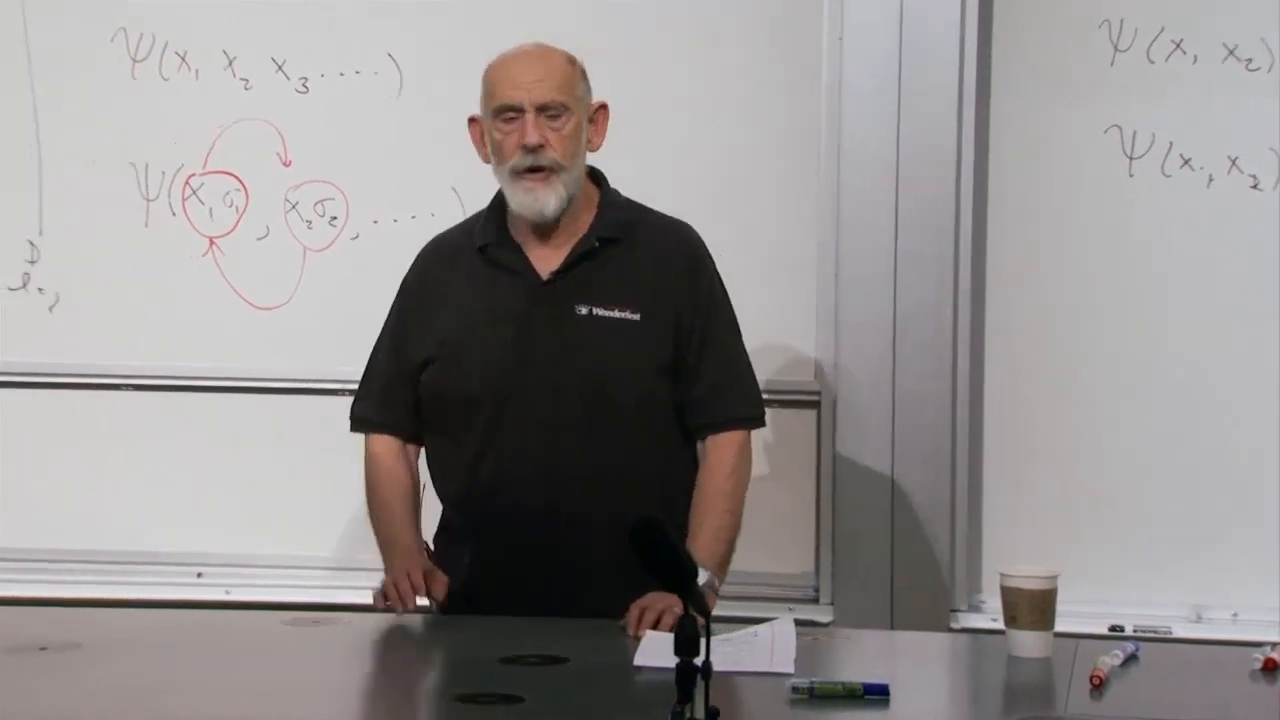
\includegraphics[width=0.9\linewidth]{lecture_05_frame_03.png}
\caption{Beim Austausch zweier identischer Teilchen werden ihre vollständigen Orts--Spin-Bezeichnungen vertauscht. Ein bosonischer Zustand bleibt unverändert, während ein fermionischer sein Vorzeichen ändert.}
\lectureframe{00:35:25}
\end{figure}

Hier kommen zwei verschiedene Arten von Linearität zum Einsatz. Für ein Teilchen ist
\begin{equation}
\alpha\psi_0(x)+\beta\psi_1(x)
\end{equation}
eine Superposition zweier Alternativen. Für zwei Teilchen ist
\begin{equation}
\psi_0(x_1)\psi_1(x_2)
\end{equation}
eine Produktamplitude in einem Raum mit zwei Teilchenkoordinaten. Durch Symmetrisierung oder Antisymmetrisierung wird dieses Produkt mit seinem vertauschten Gegenstück kombiniert.

\begin{classroomqa}
\lecturetimestamp{00:36:13}
\audiencequestion{Führt der Teilchenaustausch zu einem Interferenzeffekt?}
\lecturerresponse{Ja. Die verschwindende fermionische Amplitude für denselben Zustand lässt sich als destruktive Interferenz der beiden ausgetauschten Beiträge verstehen.}
\end{classroomqa}

\begin{classroomqa}
\lecturetimestamp{00:37:13}
\audiencequestion{Hat Pauli den Ausschluss mithilfe desselben Symmetriearguments hergeleitet?}
\lecturerresponse{Pauli ging von einer empirischen Tatsache aus und fand einen mathematischen Rahmen, in dem sie sich ausdrücken ließ. Zunächst leitete er den Ausschluss nicht aus einer fundamentaleren Theorie her.}
\end{classroomqa}

Die Antisymmetrie liefert den mathematischen Rahmen, in dem sich die empirische Ausschlussregel ausdrücken lässt.

\begin{classroomqa}
\lecturetimestamp{00:39:01}
\audiencequestion{Hängt die Interferenz beim Teilchenaustausch mit der Interferenz zwischen alternativen Wegen zusammen?}
\lecturerresponse{Ja. In einer möglichen Geschichte passieren die beiden Teilchen einander, ohne sich zu kreuzen; in einer anderen kreuzen sie sich und gelangen so zu den vertauschten Endorten. Bei Bosonen addieren sich die Amplituden, bei Fermionen können sie sich auslöschen.}
\end{classroomqa}

Der Austausch liefert das erste Minuszeichen. Die Rotation liefert das zweite.

\section{Das zweite Minuszeichen: Rotation um \texorpdfstring{\(2\pi\)}{2 pi}}

Eine vollständige Rotation scheint nichts zu bewirken. Jede gewöhnliche geometrische Richtung kehrt nach einem Winkel von \(2\pi\) zu ihrer Ausgangslage zurück. Zurückkehren müssen jedoch die Wahrscheinlichkeiten und Erwartungswerte. Der Zustandsvektor selbst kann mit einer globalen Phase zurückkehren, ebenso wie beim Austausch.

\begin{classroomqa}
\lecturetimestamp{00:42:12}
\audiencequestion{Um welche Achse wird rotiert, und ist der Generator der Bahndrehimpuls, der Spin oder beides?}
\lecturerresponse{Man kann eine äußere Achse wählen; im Folgenden nehmen wir die \(z\)-Achse. Der Generator ist der Gesamtdrehimpuls, einschließlich der orbitalen und der Spinbeiträge. Der Spin selbst muss nicht entlang der gewählten Achse zeigen.}
\end{classroomqa}

\editorialnote{In dieser Diskussion werden die Formeln für den Drehimpuls mit \(\hbar=1\) geschrieben; \(m\) ist daher der dimensionslose Eigenwert von \(J_z\).}

Sei \(\psi(\theta)\) der Zustand, der entsteht, wenn der Rotationsparameter einen Winkel von \(\theta\) durchläuft. In der hier verwendeten Konvention gilt
\begin{equation}
J_z\psi(\theta)
=
-i\frac{\partial}{\partial\theta}\psi(\theta).
\end{equation}
Für einen Zustand mit bestimmtem \(J_z\) gilt
\begin{equation}
J_z\psi(\theta)=m\psi(\theta).
\end{equation}
Durch Kombination der Gleichungen erhält man
\begin{equation}
-i\frac{\partial}{\partial\theta}\psi(\theta)
=
m\psi(\theta),
\end{equation}
mit der Lösung
\begin{equation}
\psi(\theta)=e^{im\theta}\psi(0).
\end{equation}

Die zulässigen Werte von \(m\) sind ganzzahlig oder halbzahlig. Daher gilt
\begin{equation}
\psi(2\pi)
=
\begin{cases}
+\psi(0), & m\in\mathbb Z,\\[4pt]
-\psi(0), & m\in\mathbb Z+\tfrac12.
\end{cases}
\end{equation}
Nach einer weiteren vollständigen Drehung gilt in beiden Fällen
\begin{equation}
\psi(4\pi)=\psi(0)
\end{equation}
Dies ist das zweite Minuszeichen: Ein Zustand aus einem Drehimpulsmultiplett mit halbzahligem Drehimpuls ändert bei einer Rotation um \(2\pi\) sein Vorzeichen.

Das Vorzeichen ändert \(\lvert\psi\rvert^2\) nicht und bleibt daher unsichtbar, wenn es den gesamten Zustand multipliziert. Dennoch wird eine Rotation um \(2\pi\) bei einem Zustand mit halbzahligem Spin nicht durch die Identität dargestellt. Beobachtbar wird der Unterschied, wenn das Vorzeichen relativ zu einer anderen kohärenten Amplitude auftritt.

\section{Die Wege mit \texorpdfstring{\(2\pi\) und \(4\pi\)}{2 pi und 4 pi}}

Der Unterschied zwischen \(2\pi\) und \(4\pi\) lässt sich ohne weitere Algebra sichtbar machen. Halten Sie eine Tasse in einer Hand und drehen Sie sie um eine volle Umdrehung, ohne sie loszulassen. Die Tasse kehrt in ihre ursprüngliche Ausrichtung zurück, aber der Arm ist verdreht. Drehen Sie sie eine weitere Umdrehung, lässt sich der Arm in seine ursprüngliche Lage zurückbringen, ohne die Drehbewegung der Tasse umzukehren.

Eine verwandte Konstruktion verwendet eine Kugel in einer Schachtel, die mit Schnüren an der Schachtel befestigt ist. Dreht man die Kugel um \(2\pi\), entsteht ein Wirrwarr. Im gewöhnlichen dreidimensionalen Raum lässt sich das Gewirr, das einer Drehung um \(4\pi\) entspricht, entwirren. Entscheidend ist nicht nur die Endausrichtung der Kugel, sondern der Weg durch den Raum der Rotationen.

\begin{classroomqa}
\lecturetimestamp{00:54:22}
\audiencequestion{Wenn die Kugel zweimal um dieselbe Achse gedreht wird, lassen sich die Schnüre dann wirklich entwirren? Erfordert das eine weitere räumliche Dimension?}
\lecturerresponse{Der Weg mit \(4\pi\) lässt sich im gewöhnlichen dreidimensionalen Raum entwirren. Die Zeit parametrisiert die Bewegung; sie ist keine weitere räumliche Richtung. Ein Weg mit \(2\pi\) lässt sich auf diese Weise nicht entwirren, ein Weg mit \(4\pi\) dagegen schon.}
\end{classroomqa}

Die Demonstrationen unterscheiden einen nichttrivialen Weg mit \(2\pi\) von einem entwirrbaren Weg mit \(4\pi\), ohne eine formale Theorie der Rotationsgruppe zu entwickeln.

\section{Austausch und Rotation im Gürtelbild}

Nun stehen die beiden Minuszeichen nebeneinander. Der Austausch zweier identischer Fermionen ändert das Vorzeichen ihrer gemeinsamen Wellenfunktion. Auch eine Rotation eines Zustands mit halbzahligem Spin um \(2\pi\) ändert sein Vorzeichen. Ein Gürtel stellt eine geometrische Beziehung zwischen diesen beiden Vorgängen her.

Ordnen Sie den Gürtel so an, dass seine beiden unteren Enden vertauscht sind. Anders betrachtet weist derselbe Gürtel eine Verdrehung um \(2\pi\) auf. Führt man den Austausch zusammen mit der Rotation um \(2\pi\) aus, verschwindet die Verdrehung und der Gürtel bleibt unverdrillt. Der kombinierte Vorgang lässt sich stetig auf nichts tun zurückführen.\footnote{Die Beobachtung zum Austausch und zur--Rotation wird in der Vorlesung David Finkelstein zugeschrieben. Da die Quellenaufzeichnung keine bestimmte Veröffentlichung nennt, wird der Name hier nur als diese Zuschreibung beibehalten.}

\begin{classroomqa}
\lecturetimestamp{01:01:12}
\audiencequestion{Beschreibt dies nur die Einbettung des Gürtels in den Raum oder auch die Topologie von Teilchen?}
\lecturerresponse{Der Gürtel lässt sich als Teilchengeschichte in der Raumzeit auffassen. Zeigt die Zeit nach oben, liefert ein Querschnitt teilchenartige Objekte. Paare werden erzeugt, ein Objekt wird um \(2\pi\) gedreht und zwei identische Objekte werden vertauscht. In dieser Geschichte heben sich die Rotations- und Austauschphasen auf.}
\end{classroomqa}

An dieser Geschichte lässt sich die Phasenbilanz explizit ablesen. Beginnen wir ohne Teilchen. An zwei voneinander getrennten Orten wird jeweils ein Teilchen--Antiteilchen-Paar erzeugt, sodass es zu einem Zwischenzeitpunkt vier Teilchen gibt. Während ein Teilchen um \(2\pi\) gedreht wird, werden an anderer Stelle in der Konfiguration zwei identische Teilchen vertauscht. Die vollständige Geschichte lässt sich in die elementare Geschichte umformen, in der ein Paar erzeugt und später wieder vernichtet wird. In der hier betrachteten Vorzeichenbilanz hat diese triviale Geschichte keine zusätzliche Phase. Bezeichnen \(\eta_{\mathrm{rot}}\) und \(\eta_{\mathrm{ex}}\) die beiden Vorzeichen, lässt sich die mündlich beschriebene Aufhebung knapp so schreiben:\footnote{Diese Phasengleichung hält die Aufhebung fest, die von 01:06:50 bis 01:07:18 beschrieben wird; die Vorlesung stellt die Konstruktion als anschaulich, nicht als strengen Beweis dar.}
\begin{equation}
\eta_{\mathrm{rot}}\eta_{\mathrm{ex}}=1.
\end{equation}

\begin{classroomqa}
\lecturetimestamp{01:03:34}
\audiencequestion{Lässt sich der Austausch mit Rotationen verknüpfen, indem sich beide Teilchen um \(\pi\) bewegen und anschließend neu ausrichten?}
\lecturerresponse{Diese Konstruktion könnte verwandte Mathematik widerspiegeln, verwendet aber zwei getrennte Rotationen um \(\pi\). Der hier analysierte Vorgang umfasst eine Rotation um \(2\pi\); die beiden Argumente sind also nicht identisch.}
\end{classroomqa}

Das Argument setzt voraus, dass teilchenartige Objekte erzeugt und vernichtet werden können. In einer Theorie mit ewigen Teilchen hätte es nicht diese Form. Es wird auch nicht als Standardbeweis des Spin--Statistik-Theorems vorgelegt. Es soll einen topologischen Grund dafür veranschaulichen, dass die Vorzeichen von Austausch und Rotation zusammenpassen.

\section{Klumpen, Spiegelbilder und Vernichtung}

Die Konstruktion lässt sich mit lokalisierten Feldkonfigurationen wiederholen. Nehmen wir an, ein oder mehrere Felder nehmen fast überall ihre Vakuumwerte an, weisen aber in einem kleinen Bereich eine nichtverschwindende Form und Struktur auf. Eine solche lokalisierte Konfiguration ist ein Klumpen.

Erzeugen wir nun eine zweite Konfiguration als das passende Spiegelbild der ersten. Nennen wir die eine Teilchen und die andere Antiteilchen. Bringen wir sie zusammen. Entsprechende Teile der Feldkonfigurationen treffen aufeinander und heben sich gegenseitig auf. In einem Zwischenstadium können manche Teile der Klumpen bereits verschwunden sein, während andere noch bestehen. Durch Fortsetzen der Verformung verschwindet auch die übrige Struktur, und die Felder kehren zur Vakuumkonfiguration zurück. Zwei entgegengesetzt angeordnete Verdrehungen in einem Gürtel veranschaulichen dasselbe: Schiebt man sie zusammen, entwirren sie sich.

Der Vorgang lässt sich rückwärts ablaufen. Aus dem leeren Raum können ein Klumpen und sein Spiegelbild entstehen. Man kann zwei solcher Paare erzeugen, einen Klumpen um \(2\pi\) drehen, zwei identische Klumpen vertauschen und die Paare wieder vernichten. Dieselbe Aufhebung von Austausch und--Rotation gilt dann auch hier. Dies bleibt eine heuristische Erweiterung der Konstruktion und ist kein Theorem über jede lokalisierte Anregung.

\begin{classroomqa}
\lecturetimestamp{01:11:30}
\audiencequestion{Gibt es physikalische Realisierungen solcher klumpenartigen Feldkonfigurationen?}
\lecturerresponse{Ja. Beispiele sind Kerne in Skyrmion-artigen Beschreibungen, magnetische Monopole und andere teilchenartige Anregungen von Feldern.}
\end{classroomqa}

Das Bild der gespiegelten Klumpen macht die Verallgemeinerung verständlich. Entscheidend ist nicht, dass das Objekt ursprünglich ein elementares Punktteilchen war, sondern dass eine teilchenartige Anregung und ihr Partner kontinuierlich erzeugt, zusammengebracht und vernichtet werden können. Diese Eigenschaft legt eine allgemeinere Beziehung zwischen Rotations- und Austauschverhalten nahe.

\begin{classroomqa}
\lecturetimestamp{01:16:12}
\audiencequestion{Bedeutet Spin eins halb, dass der Zustand nur die Hälfte der üblichen Rotationsphase annimmt?}
\lecturerresponse{Die Phase lautet in dieser Konvention \(e^{im\theta}\). Für halbzahliges \(m\) ergibt eine Rotation um \(2\pi\) den Faktor \(-1\), während eine Rotation um \(4\pi\) den Faktor \(+1\) ergibt.}
\end{classroomqa}

\section{Ein globales Vorzeichen und ein Nullresultat}

Lässt sich das Minuszeichen einer Rotation um \(2\pi\) beobachten? Beginnen wir mit einem Experiment, bei dem das nicht möglich ist. Fangen wir ein Elektron in einem Magnetfeld ein, lassen seinen Spin dem Feld folgen, während die Apparatur langsam um \(2\pi\) gedreht wird, und geben das Elektron anschließend in eine Interferenzapparatur frei. Vergleichen wir dies mit demselben Ablauf ohne Rotation.

Die Rotation verändert den Zustand gemäß
\begin{equation}
\psi\longmapsto-\psi,
\end{equation}
Doch das Minuszeichen multipliziert den gesamten Zustand. Alle Wahrscheinlichkeiten bleiben unverändert; das abschließende Interferenzmuster enthält daher keine Information darüber, ob die vorherige Rotation stattgefunden hat. Dies ist ein Nullresultat: Eine gemeinsame Phase hat nichts, womit sie interferieren könnte.

\begin{classroomqa}
\lecturetimestamp{01:20:01}
\audiencequestion{Warum muss die Drehung des Magnetfelds langsam erfolgen?}
\lecturerresponse{Der Spin muss dem rotierenden Magnetfeld weiter folgen. Wird das Feld zu schnell bewegt, bleibt der Spin nicht an es gekoppelt.}
\end{classroomqa}

\section{Ein Elektron in zwei kohärenten Zweigen}

Das Vorzeichen wird beobachtbar, wenn man es relativ macht. Schicken wir ein Elektron durch einen Strahlteiler. Ein Teil seiner Wellenfunktion folgt dem einen Weg, ein anderer Teil einem zweiten:
\begin{equation}
\psi(x)=\psi_1(x)+\psi_2(x).
\end{equation}
Es handelt sich um ein Elektron, nicht um zwei Elektronen. Es ist eine kohärente Superposition zweier Alternativen. Diese Unterscheidung muss klar bleiben: Die beiden Wellenpakete sind keine zwei unabhängigen Teilchen.

Führen wir die beiden Wellenpakete in getrennte Bereiche mit Magnetfeldern. Drehen wir das Feld in einem Bereich um \(2\pi\) und lassen das andere unverändert. Für einen Zustand mit halbzahligem Spin gilt
\begin{equation}
\psi_1(x)+\psi_2(x)
\longmapsto
\psi_1(x)-\psi_2(x),
\end{equation}
wobei der gedrehte Zweig mit \(2\) bezeichnet wird. Nun ist das Vorzeichen relativ. Wenn sich die beiden Wellenpakete später überlagern, wird aus der Addition eine Subtraktion. Ein Punkt konstruktiver Interferenz kann zu einem Punkt destruktiver Interferenz oder sogar zu einem Knoten werden.

\begin{classroomqa}
\lecturetimestamp{01:23:46}
\audiencequestion{Was wird gedreht, wenn es nur ein Elektron, aber zwei Zweige der Wellenfunktion gibt?}
\lecturerresponse{Das Elektron befindet sich in einer kohärenten Superposition zweier lokalisierter Alternativen. Ein Zweig wird gedreht, der andere nicht. Öffnet man die Kästen, um herauszufinden, welche Alternative eingetreten ist, zerstört diese Messung die Interferenz.}
\end{classroomqa}

Beim Öffnen der Kästen würde sich zeigen, dass sich das einzige Elektron in einem der beiden Kästen befindet. Ohne diese Messung bleiben beide Amplituden im Zustand erhalten. Wiederholt man das Experiment, baut sich das Interferenzmuster nach und nach auf, eine Detektion nach der anderen. An einem durch das relative Minuszeichen erzeugten Knoten wird kein Elektron detektiert.

\section{Magnetische Präzession und Doppelspaltinterferenz}

Ein praktischeres schematisches Verfahren ersetzt das sehr langsame Experiment mit den Kästen. Teilen wir eine kohärente Elektronenwelle auf zwei Wege auf. Auf einem Weg durchquert das Elektron einen Magnetfeldbereich, wobei sein Spin zunächst quer zum Feld steht. Daraufhin präzediert der Spin. Durch geeignete Wahl der Feldstärke und der Durchlaufzeit kann der Spin in diesem Zweig eine vollständige Drehung um \(2\pi\) ausführen, während der andere Zweig keine solche Drehung erfährt.\footnote{Die Vorlesung berichtet, dass ein verwandtes Spinorphasen-Experiment durchgeführt worden sei, und erläutert dessen Prinzip; die Quellenaufzeichnung nennt jedoch weder eine Veröffentlichung noch eine bestimmte Apparatur. Die Darstellung hier beschränkt sich daher auf die in der Vorlesung beschriebene Konstruktion.}

\begin{classroomqa}
\lecturetimestamp{01:27:05}
\audiencequestion{Wie lässt sich der Weg des einzelnen Elektrons bestimmen?}
\lecturerresponse{Das ist nicht möglich, ohne das Experiment zu zerstören. Jede Messung, die aufzeichnet, welchen Weg das Elektron genommen hat, zerstört die Interferenz.}
\end{classroomqa}

\begin{classroomqa}
\lecturetimestamp{01:27:50}
\audiencequestion{Was genau ist ein Zweig der Wellenfunktion, und wie erzeugt der Strahlteiler zwei Zweige?}
\lecturerresponse{Ein Zweig ist ein entlang eines Weges lokalisiertes Wellenpaket. Der Strahlteiler formt die einlaufende Welle zu zwei räumlich getrennten Wellenpaketen; elektrische oder magnetische Felder können diese auf unterschiedlichen Wegen führen.}
\end{classroomqa}

Abgesehen vom Magnetfeldbereich entspricht dies dem Doppelspaltexperiment. Eine einlaufende Elektronenwelle teilt sich in zwei Wellenpakete. Die auslaufenden Wellen breiten sich in einen gemeinsamen Detektionsbereich aus, wo sich ihre Amplituden überlagern. Ohne relative Rotation können sich die zentralen Amplituden addieren. Eine Spinrotation um \(2\pi\) auf einem der Wege kehrt eine Amplitude um und kann bewirken, dass sich dieselben Beiträge auslöschen.

\begin{classroomqa}
\lecturetimestamp{01:30:46}
\audiencequestion{Wie kann es Interferenz geben, wenn das Elektron durch getrennte Röhren oder Spalte läuft?}
\lecturerresponse{Die abschließende Detektion lässt den Weg nicht erkennen. Die beiden auslaufenden Wellenamplituden breiten sich aus und überlagern sich am Detektor. Herauszufinden, welchen Weg das Elektron genommen hat, würde die Interferenz zerstören.}
\end{classroomqa}

\begin{classroomqa}
\lecturetimestamp{01:33:22}
\audiencequestion{Muss der Durchmesser der Röhre oder des Spalts in der Größenordnung der Elektronenwellenlänge liegen?}
\lecturerresponse{Bei einer wörtlichen, auf Beugung beruhenden Doppelspaltrealisierung muss die Öffnung klein genug sein, um die erforderliche Ausbreitung zu bewirken. Die beschriebene Apparatur ist schematisch und keine praktische Konstruktion.}
\end{classroomqa}

\begin{classroomqa}
\lecturetimestamp{01:33:44}
\audiencequestion{Würde eine entsprechende \(2\pi\)-Drehung der Photonenpolarisation das Interferenzmuster unverändert lassen?}
\lecturerresponse{Ja. Photonen haben ganzzahligen Spin, daher führt eine vollständige Drehung um \(2\pi\) nicht zum fermionischen Minuszeichen.}
\end{classroomqa}

\begin{classroomqa}
\lecturetimestamp{01:34:12}
\audiencequestion{Worin weicht das praktische Experiment geringfügig von der idealisierten Version ab?}
\lecturerresponse{Bei der idealisierten Anordnung wird der Spin adiabatisch gedreht. In der Beschreibung des praktischen Experiments bewegt sich das Elektron durch einen Magnetfeldbereich, und sein Spin präzediert schneller; die gemessene Phase ist jedoch weiterhin die einer Drehung um \(2\pi\).}
\end{classroomqa}

Die langsame Anordnung macht die Idee anschaulich, indem sie sicherstellt, dass der Spin dem Feld ohne zusätzliche Bewegung folgt. Bei der Präzession entsteht dasselbe relative Vorzeichen dynamisch. In beiden Versionen müssen die beiden Wege ununterscheidbar werden, bevor ein Interferenzmuster auftreten kann.

\begin{classroomqa}
\lecturetimestamp{01:36:15}
\audiencequestion{Müssen die beiden Zweige nach dem Strahlteiler wieder zusammengeführt werden?}
\lecturerresponse{Ja. Die austretenden Wellenpakete müssen sich überlappen oder sich über einen gemeinsamen Detektionsbereich ausbreiten, damit ihre Amplituden ein Interferenzmuster bilden können.}
\end{classroomqa}

\begin{classroomqa}
\lecturetimestamp{01:38:12}
\audiencequestion{Ist dieses Rotationsexperiment mit einem Elektron eine Folge des Pauli-Ausschlussprinzips?}
\lecturerresponse{Nein. Es gibt nur ein Elektron. Das Experiment misst die Spinorphase bei einer Drehung, nicht den Ausschluss zweier Fermionen aus demselben Zustand.}
\end{classroomqa}

\section{Austauschinterferenz und relative Drehung}

Ein Austauschvorzeichen ließe sich mit derselben allgemeinen Methode nachweisen, auch wenn die vorgeschlagene Apparatur komplizierter ist. Man beginnt mit zwei Elektronen und spaltet ihre gemeinsame Wellenfunktion in zwei kohärente Zweige auf. Es gibt weiterhin nur zwei Elektronen, nicht vier: Das Elektronenpaar nimmt den einen oder den anderen Weg. In einem Zweig werden die beiden Elektronen vertauscht, im anderen nicht. Nachdem die Zweige wieder zusammengeführt worden sind, zeigt sich das fermionische Austauschvorzeichen als relative Phase und kann die Interferenz verändern.

Der letzte Vorschlag vergleicht die beiden Minuszeichen direkt. Ein Zweig erhält die fermionische Austauschphase, während der andere die entsprechende Phasenänderung bei einer Drehung um \(2\pi\) erfährt. Beide Phasen sind \(-1\), daher hebt sich ihre relative Wirkung auf.\footnote{Die Aufzeichnung zwischen 01:40:26 und 01:41:15 zeigt eindeutig eine Austauschphase, eine Phasenänderung bei einer Drehung um \(2\pi\) und deren Aufhebung; die genaue Zuordnung der Drehung lässt sich aus der verfügbaren Tonaufnahme jedoch nicht rekonstruieren.} Die Vorlesung stellt dies als vorgeschlagenes Gedankenexperiment dar und sagt, dass es nach Kenntnis des Vortragenden nicht durchgeführt worden war.

\begin{classroomqa}
\lecturetimestamp{01:41:34}
\audiencequestion{Würde die Beobachtung einer Austauschphase die Ununterscheidbarkeit der beiden Elektronen infrage stellen?}
\lecturerresponse{Nein. Quantenmechanische Ununterscheidbarkeit ist subtiler als klassische Gleichheit. Sie lässt zu, dass der Zustandsvektor beim Austausch sein Vorzeichen ändert, obwohl kein beobachtbares Merkmal die Teilchen unterscheidet.}
\end{classroomqa}

Es gibt noch eine letzte Einschränkung. Eine Drehung einer gesamten isolierten Welt um \(2\pi\) ergäbe nur eine gemeinsame Phase, die sich durch kein internes Experiment nachweisen ließe. Im nachweisbaren Experiment wird ein kohärenter Zweig relativ zu einem anderen gedreht. Beobachtet wird daher kein absolutes Vorzeichen, sondern die durch ein relatives Vorzeichen erzeugte Interferenz.
